\chapter{Other Measurement Data}

\section {Participant 1}
\begin{figure}[H]
  \centering
    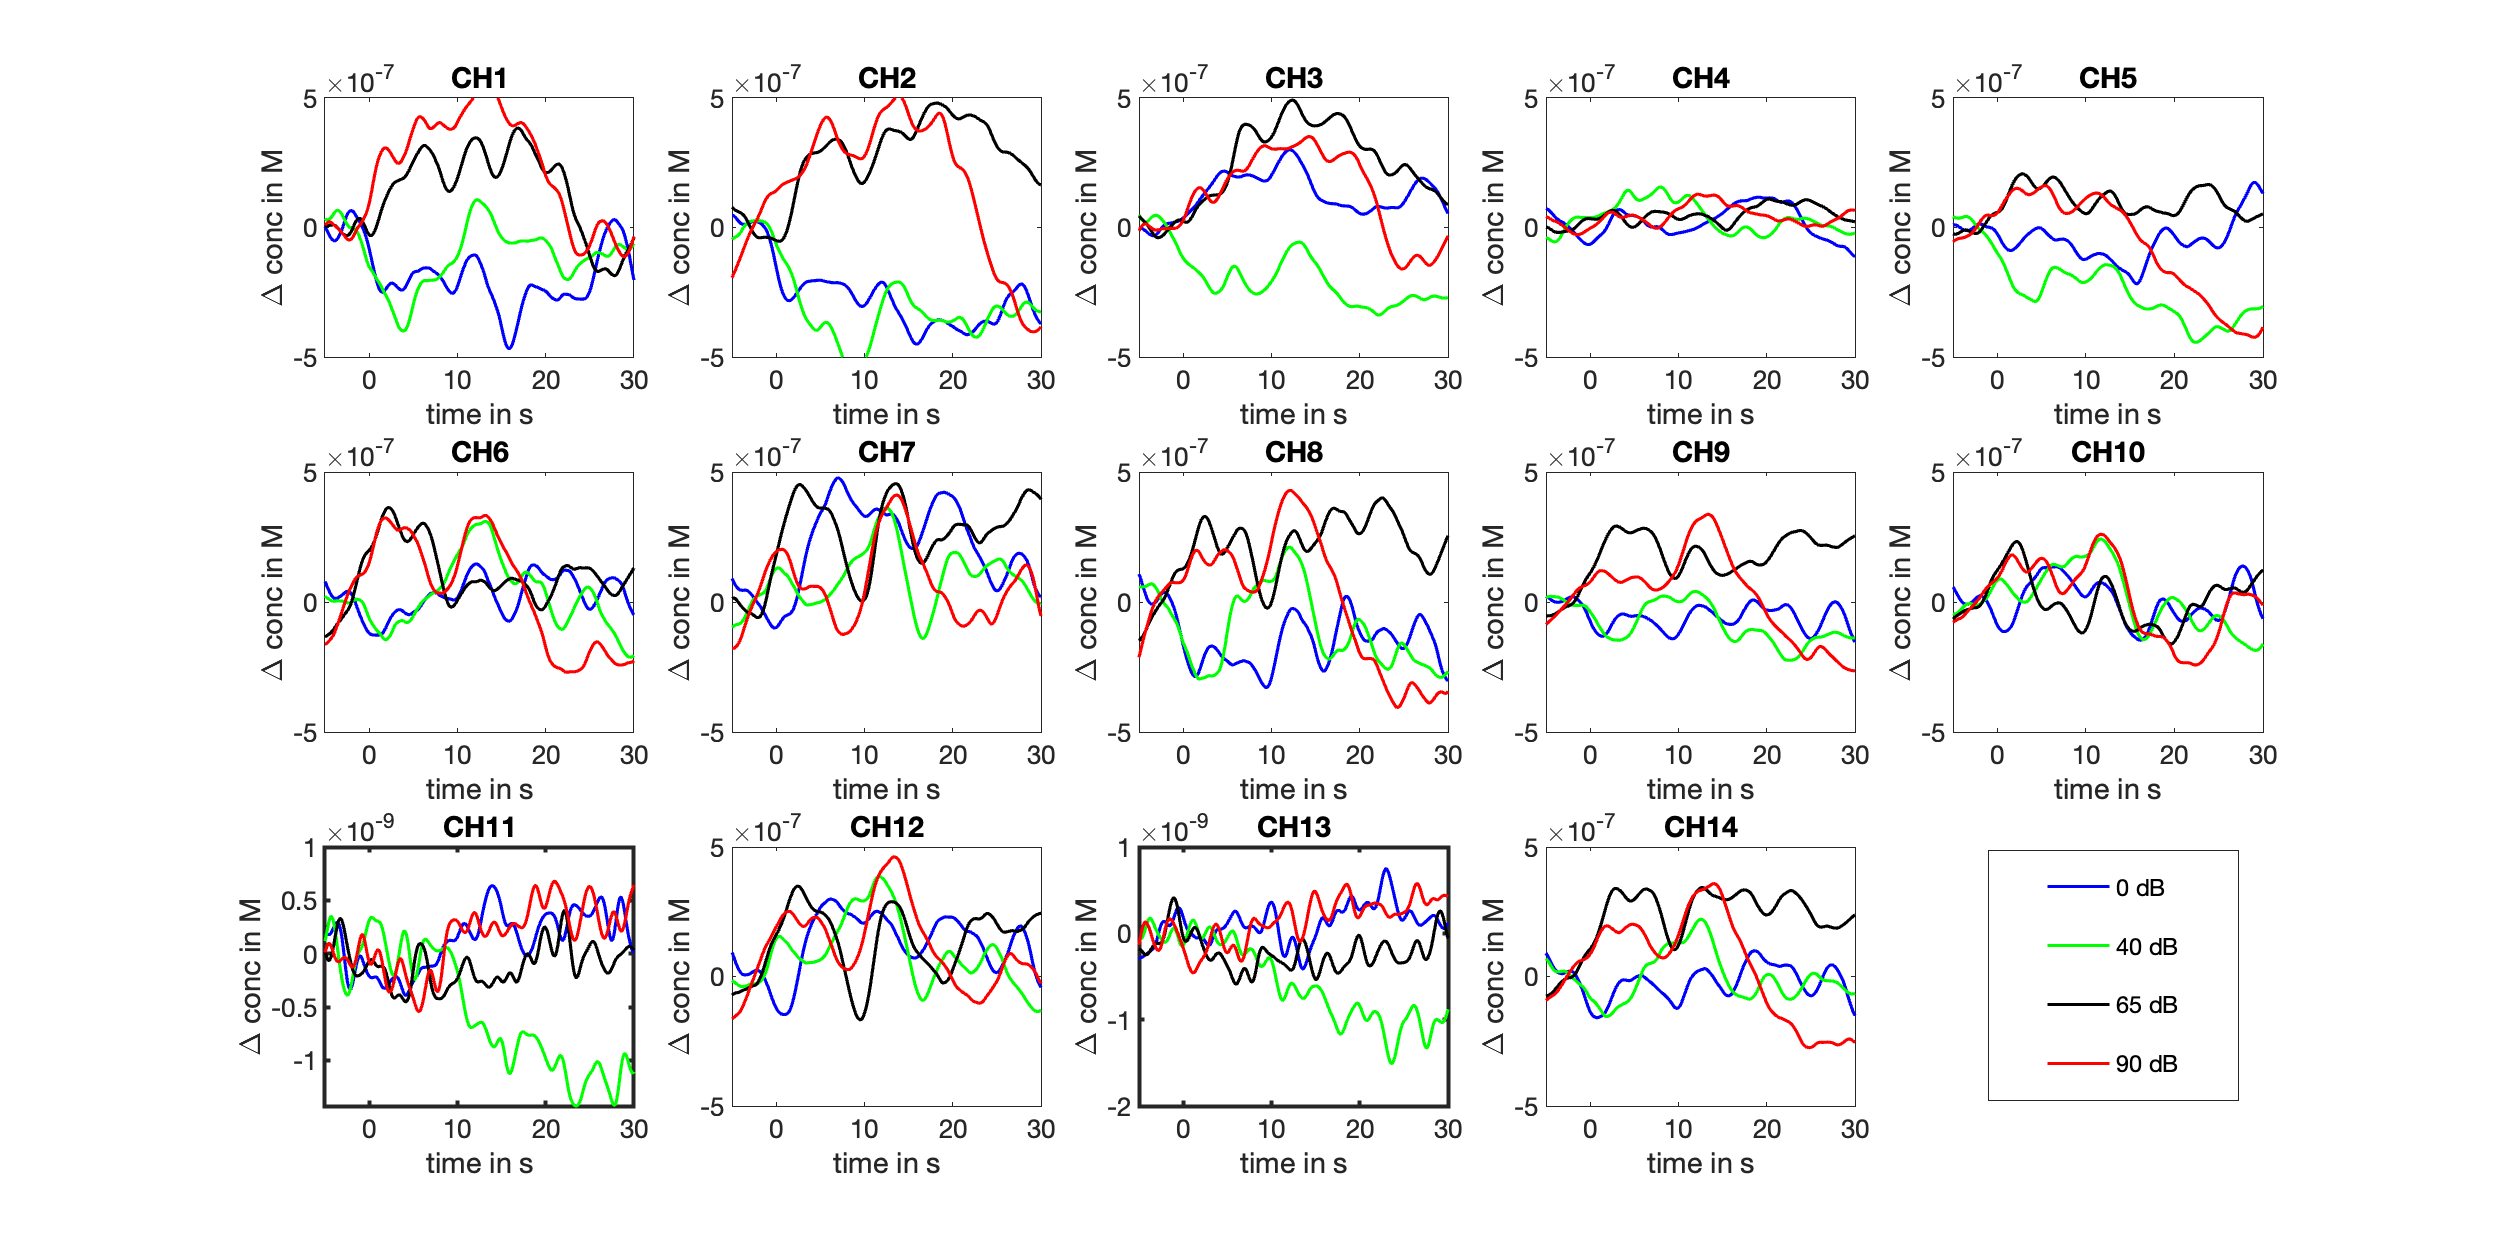
\includegraphics[scale=.4]{bilder/HbO_Mole/sub_chang_s_HbO.png}
  \caption{HbO measurement from participant 1.}
  \label{fig:somesignal}
\end{figure}

\begin{figure}[H]
  \centering
    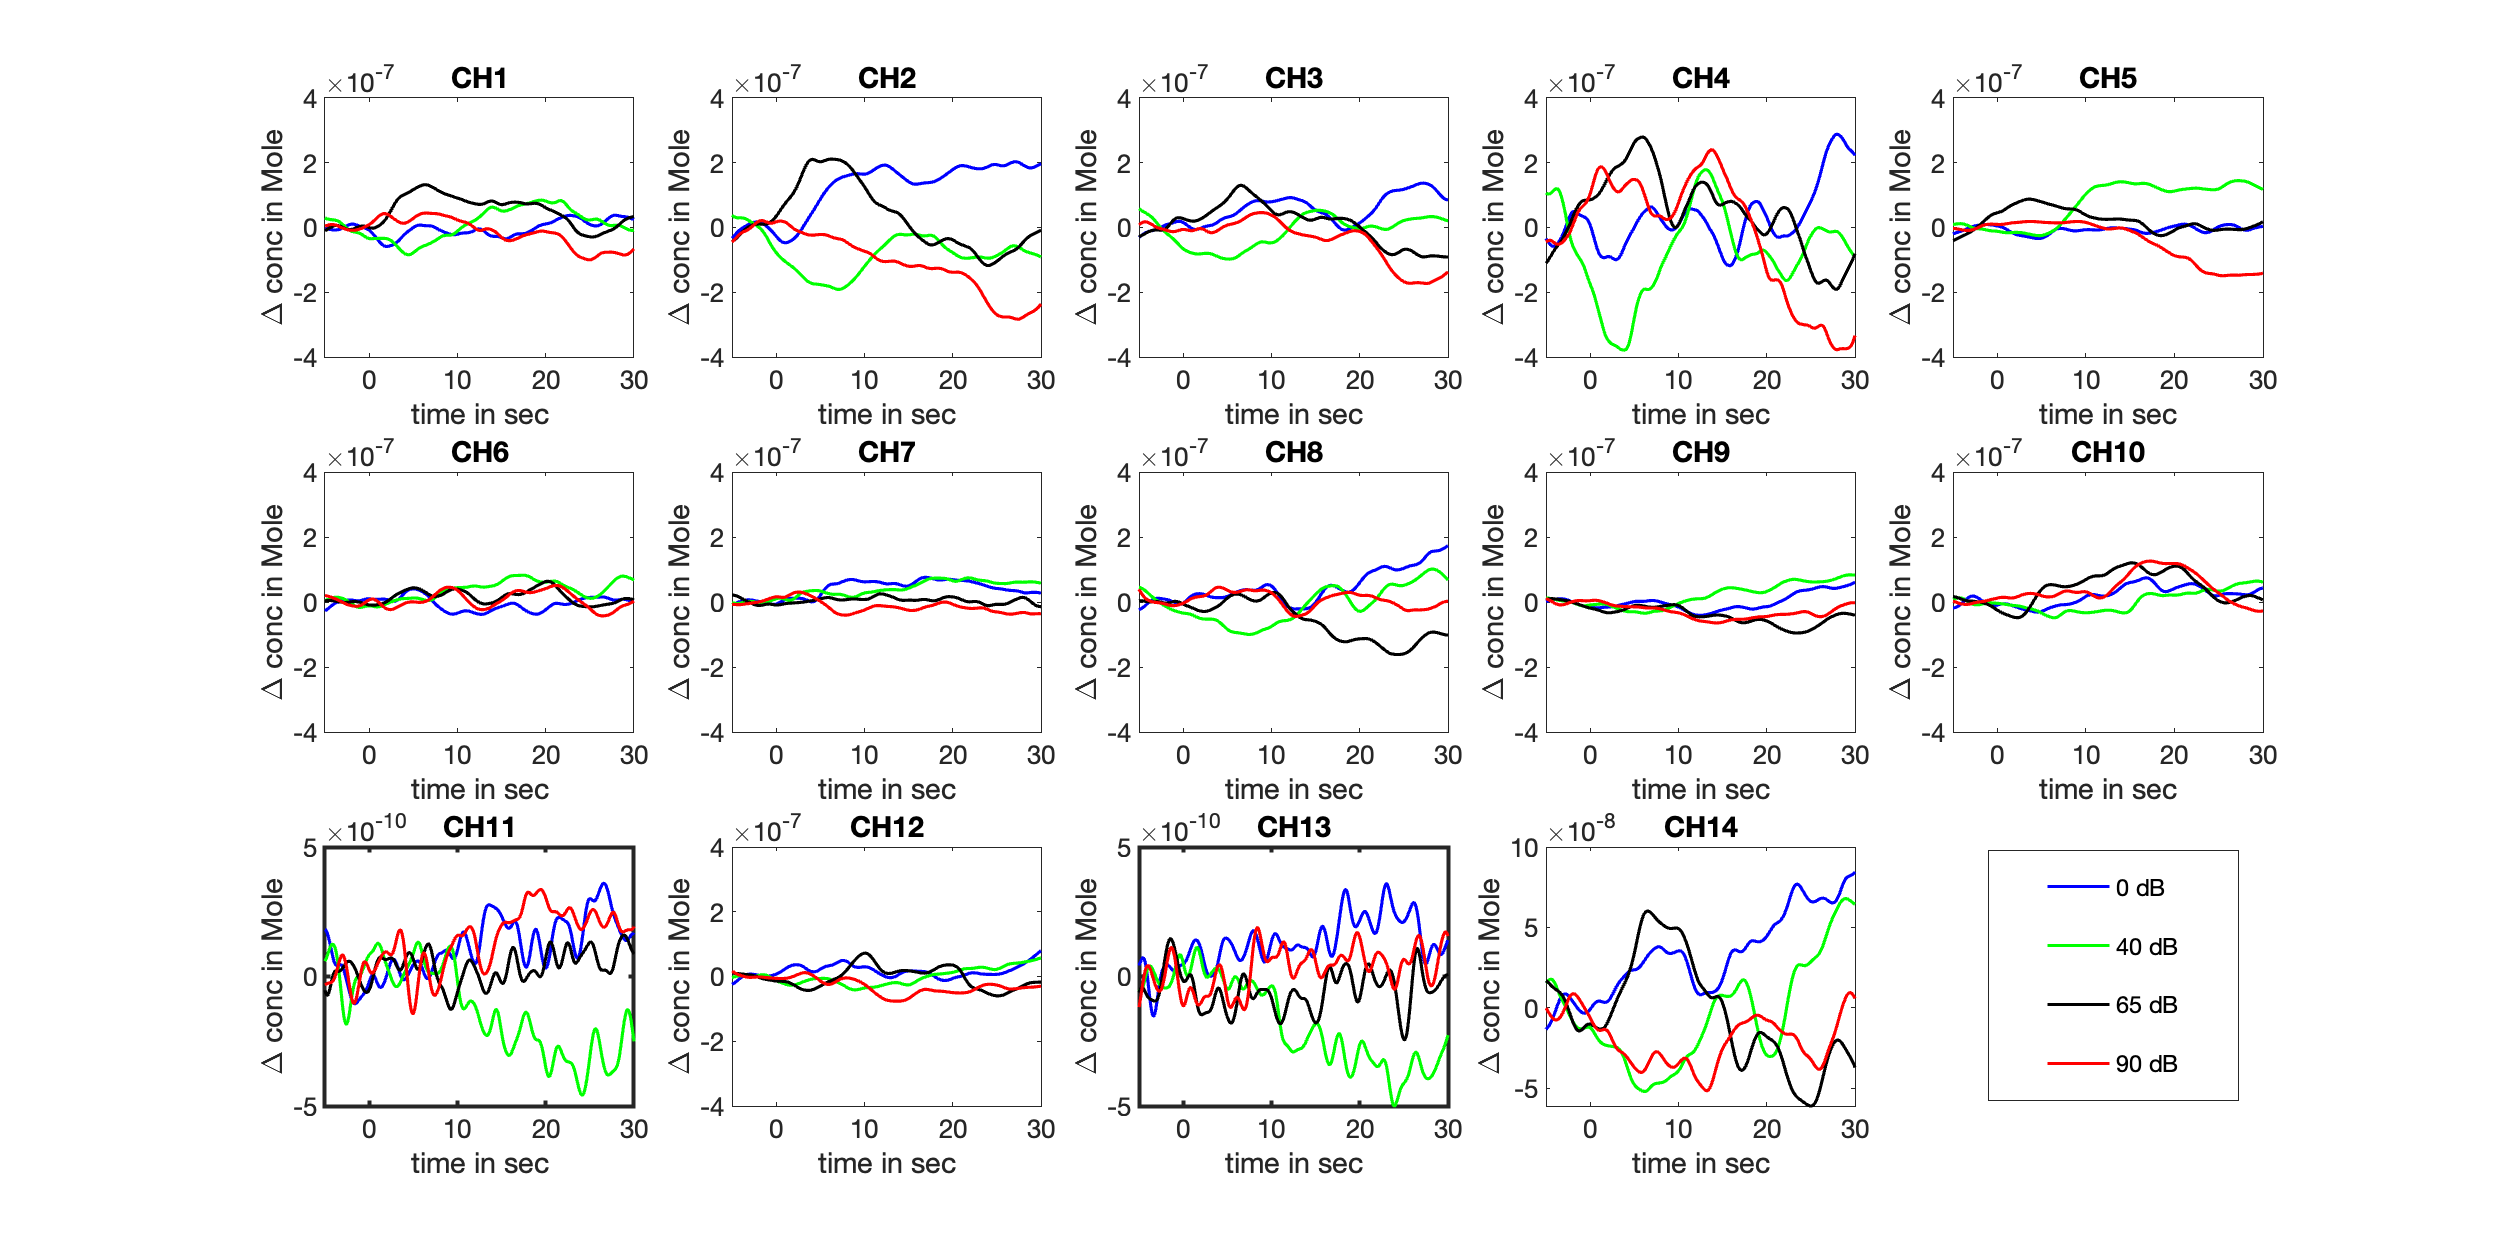
\includegraphics[scale=.4]{bilder/HbR_Mole/sub_chang_s_HbR.png}
  \caption{HbR measurement from participant 1.}
  \label{fig:somesignal}
\end{figure}

\begin{figure}[H]
  \centering
    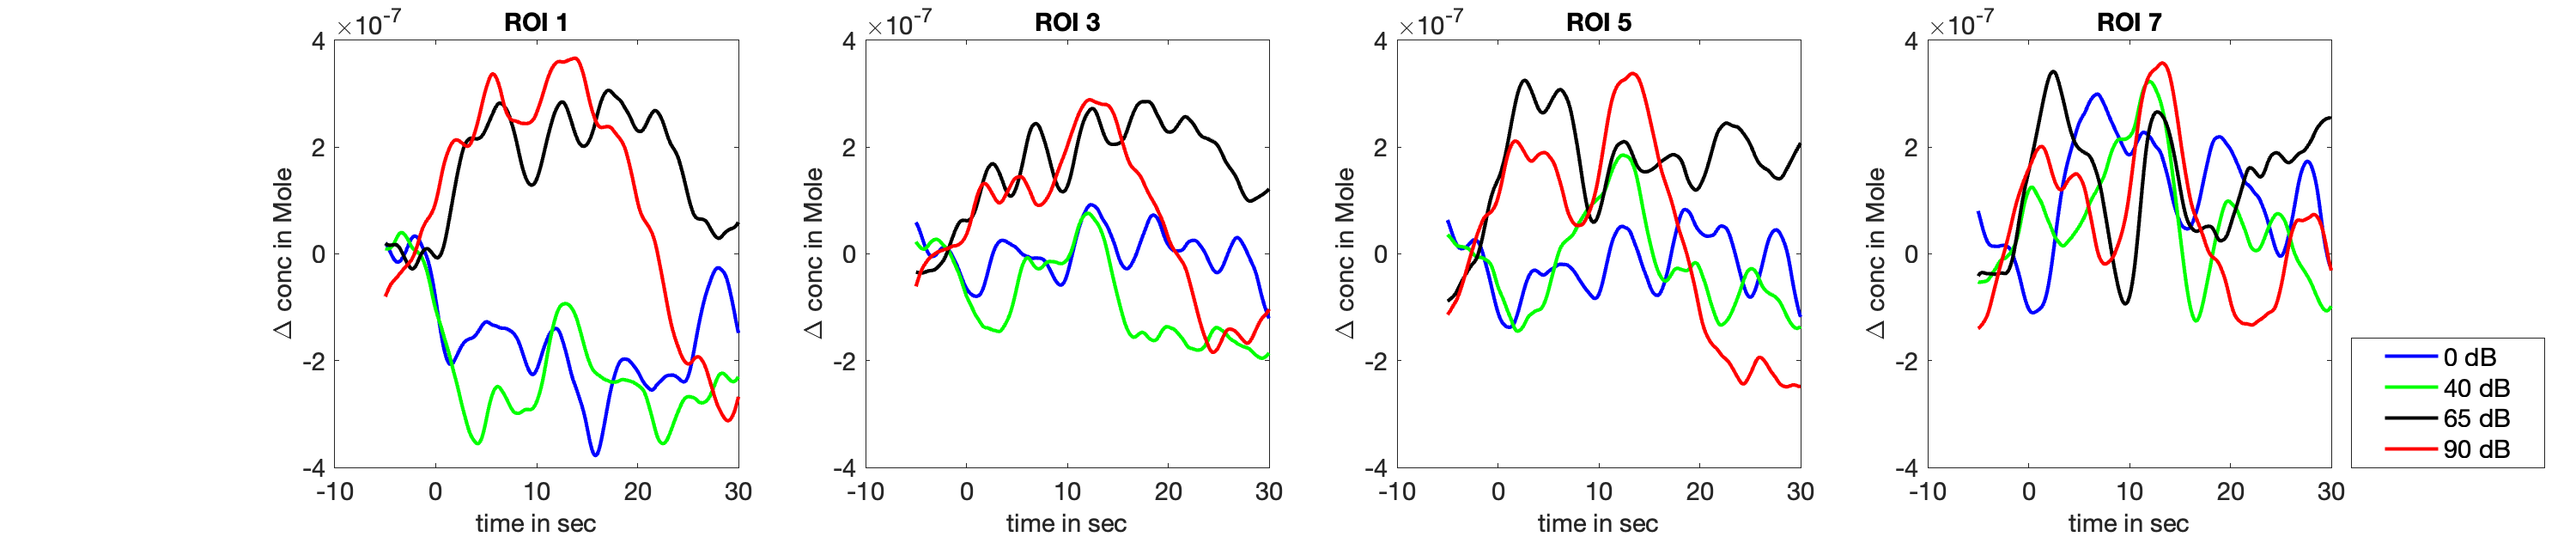
\includegraphics[scale=.29]{bilder/ROI/sub_chang_s_HbO.png}
  \caption{ROI measurement from participant 1.}
\end{figure}
\newpage


\section {Participant 2}

\begin{figure}[H]
  \centering
    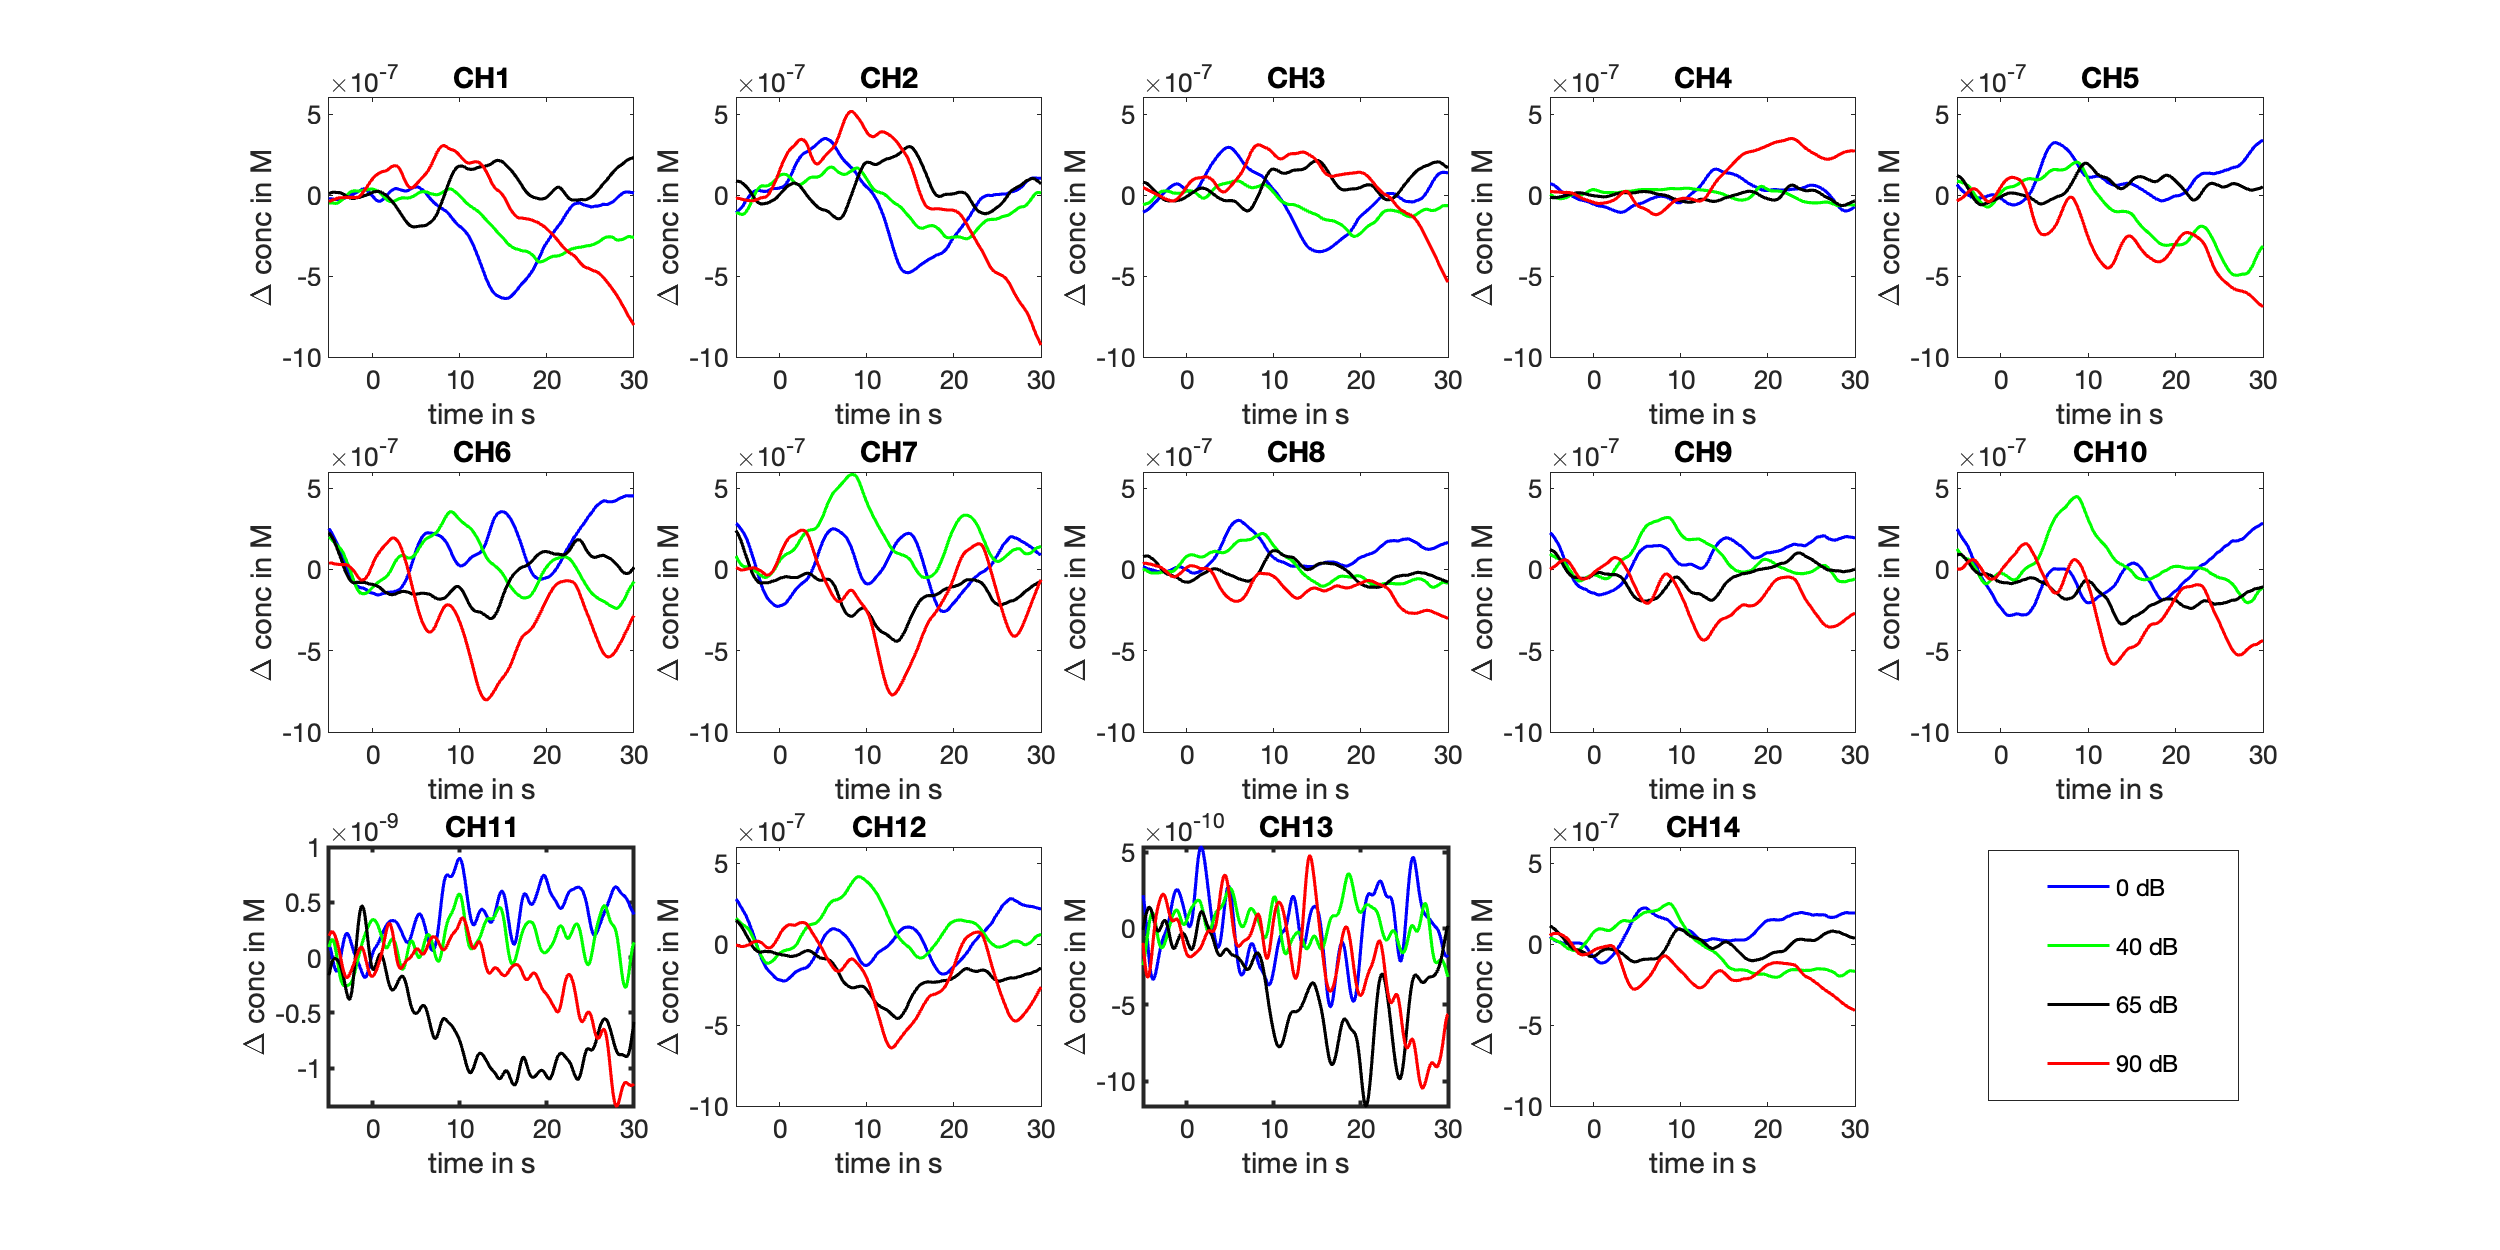
\includegraphics[scale=.4]{bilder/HbO_Mole/sub_gleb2_s_HbO.png}
  \caption{HbO measurement from participant 2.}
  \label{fig:somesignal}
\end{figure}

\begin{figure}[H]
  \centering
    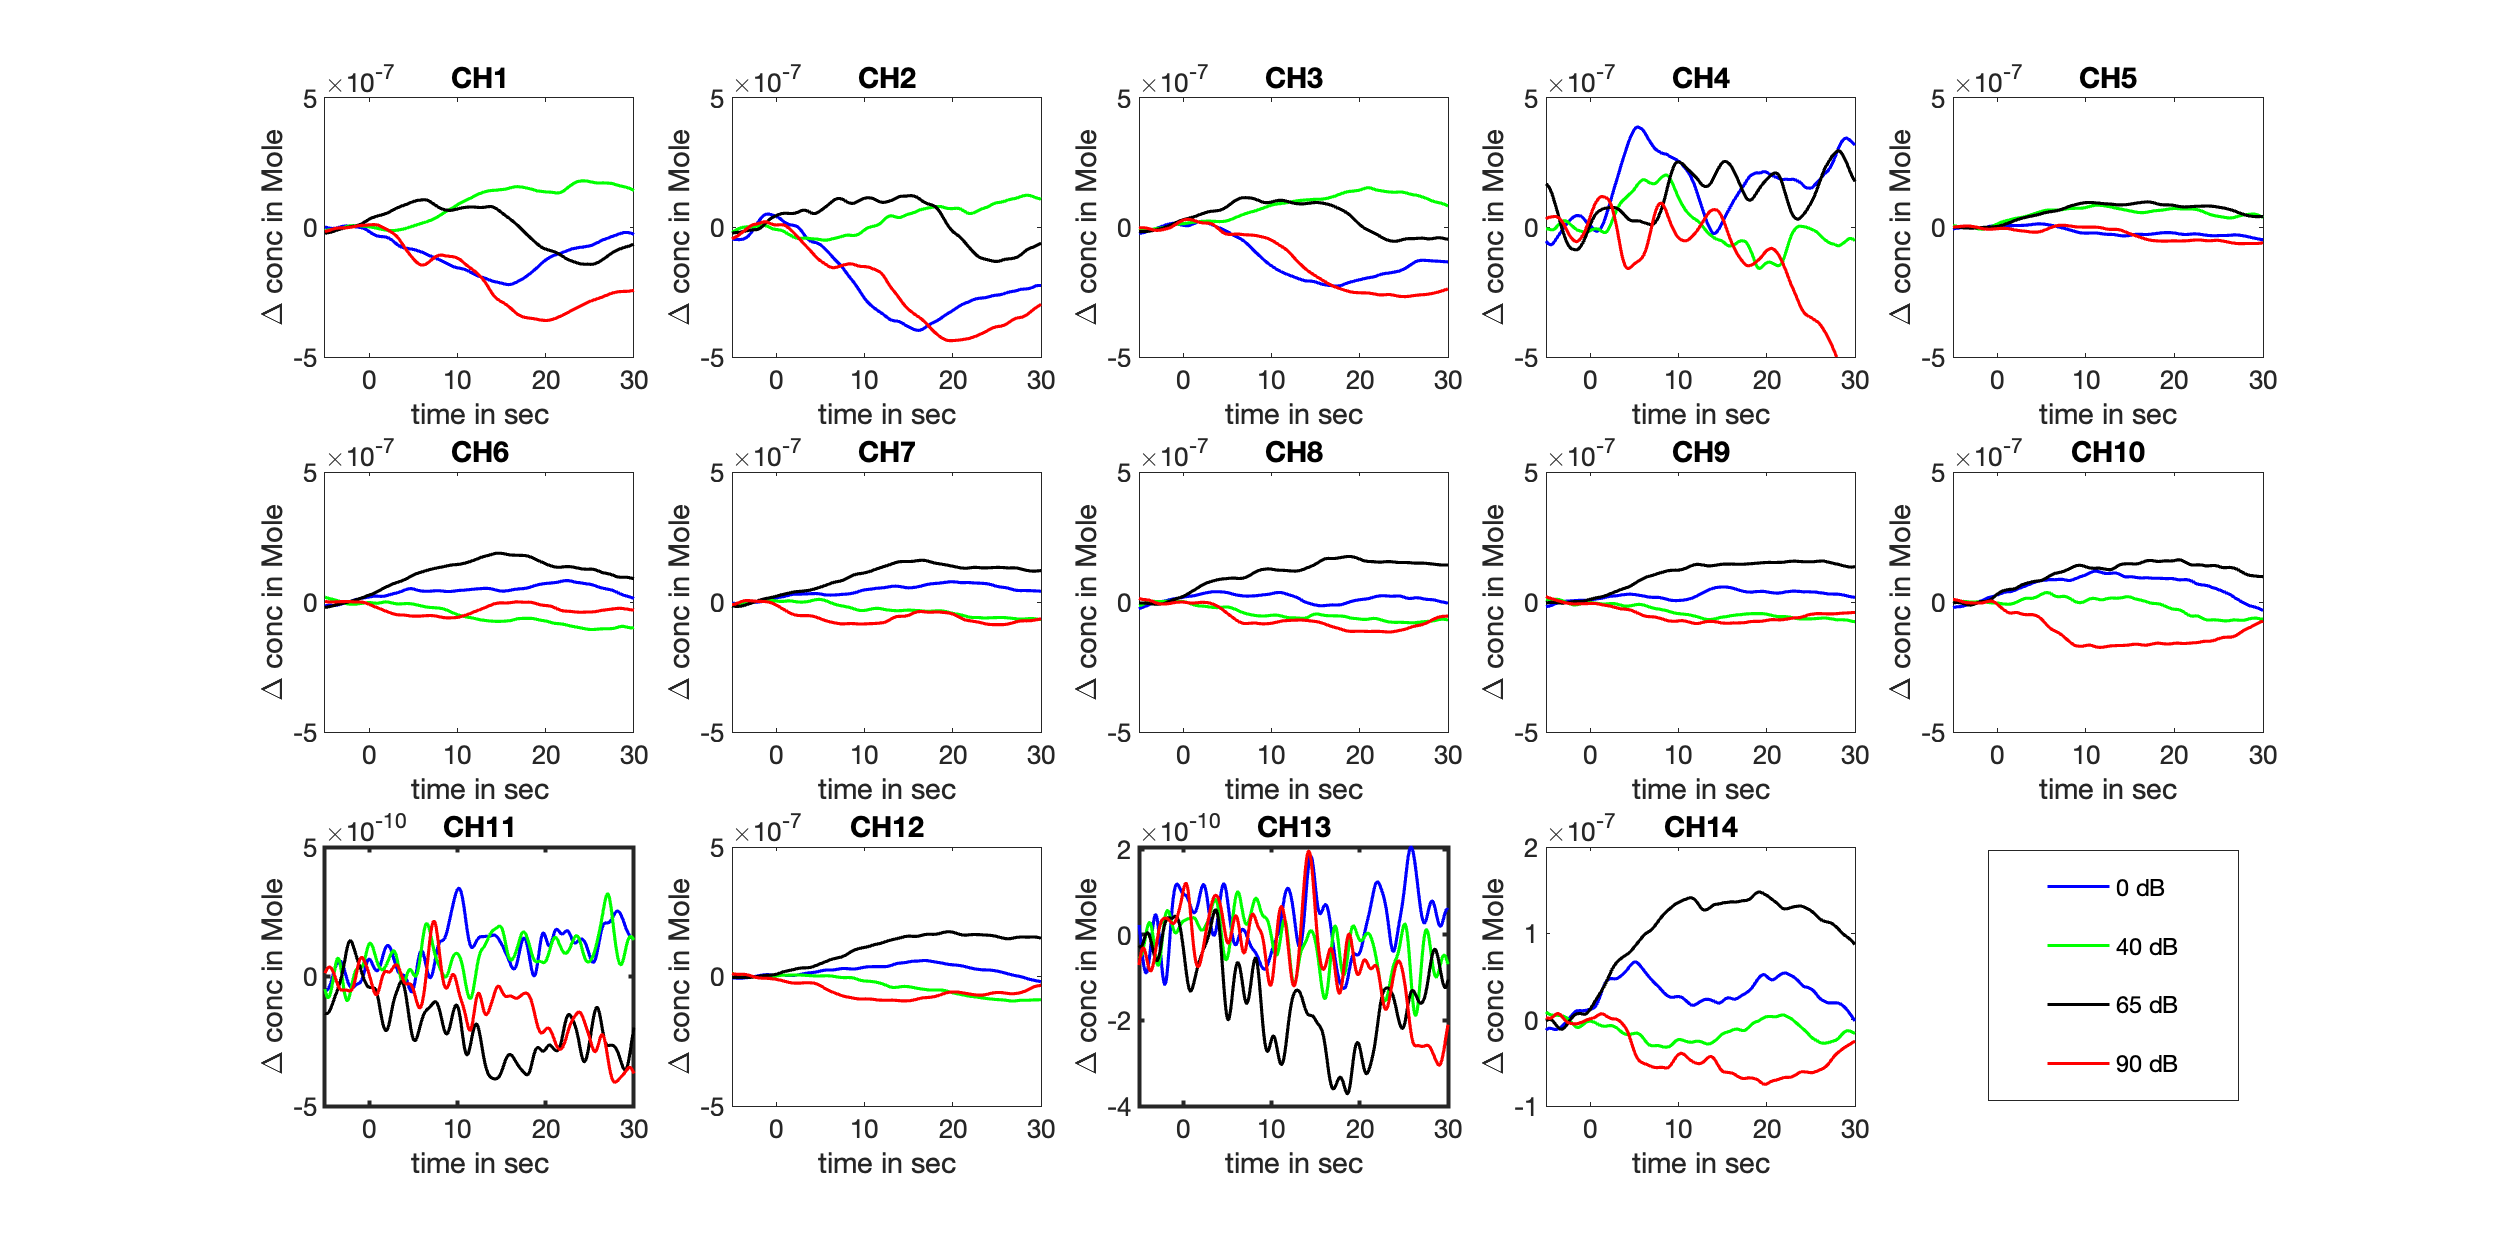
\includegraphics[scale=.4]{bilder/HbR_Mole/sub_gleb2_s_HbR.png}
  \caption{HbR measurement from participant 2.}
  \label{fig:somesignal}
\end{figure}

\begin{figure}[H]
  \centering
    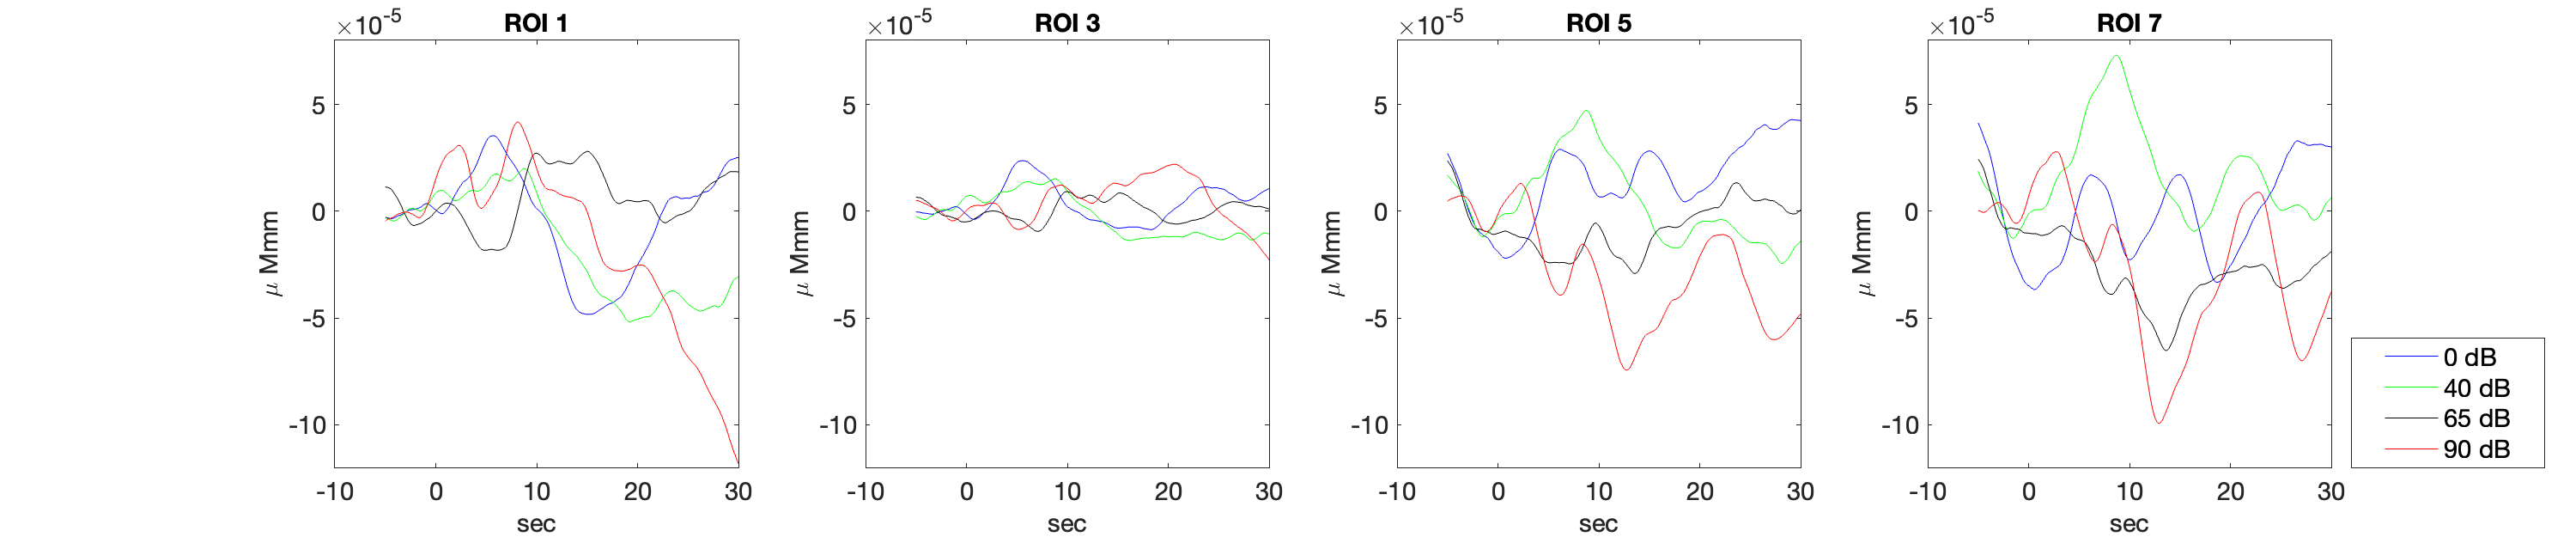
\includegraphics[scale=.29]{bilder/ROI/sub_gleb2_s_HbO.png}
  \caption{ROI measurement from participant 2.}
\end{figure}

\newpage


\section {Participant 8}

\begin{figure}[H]
  \centering
    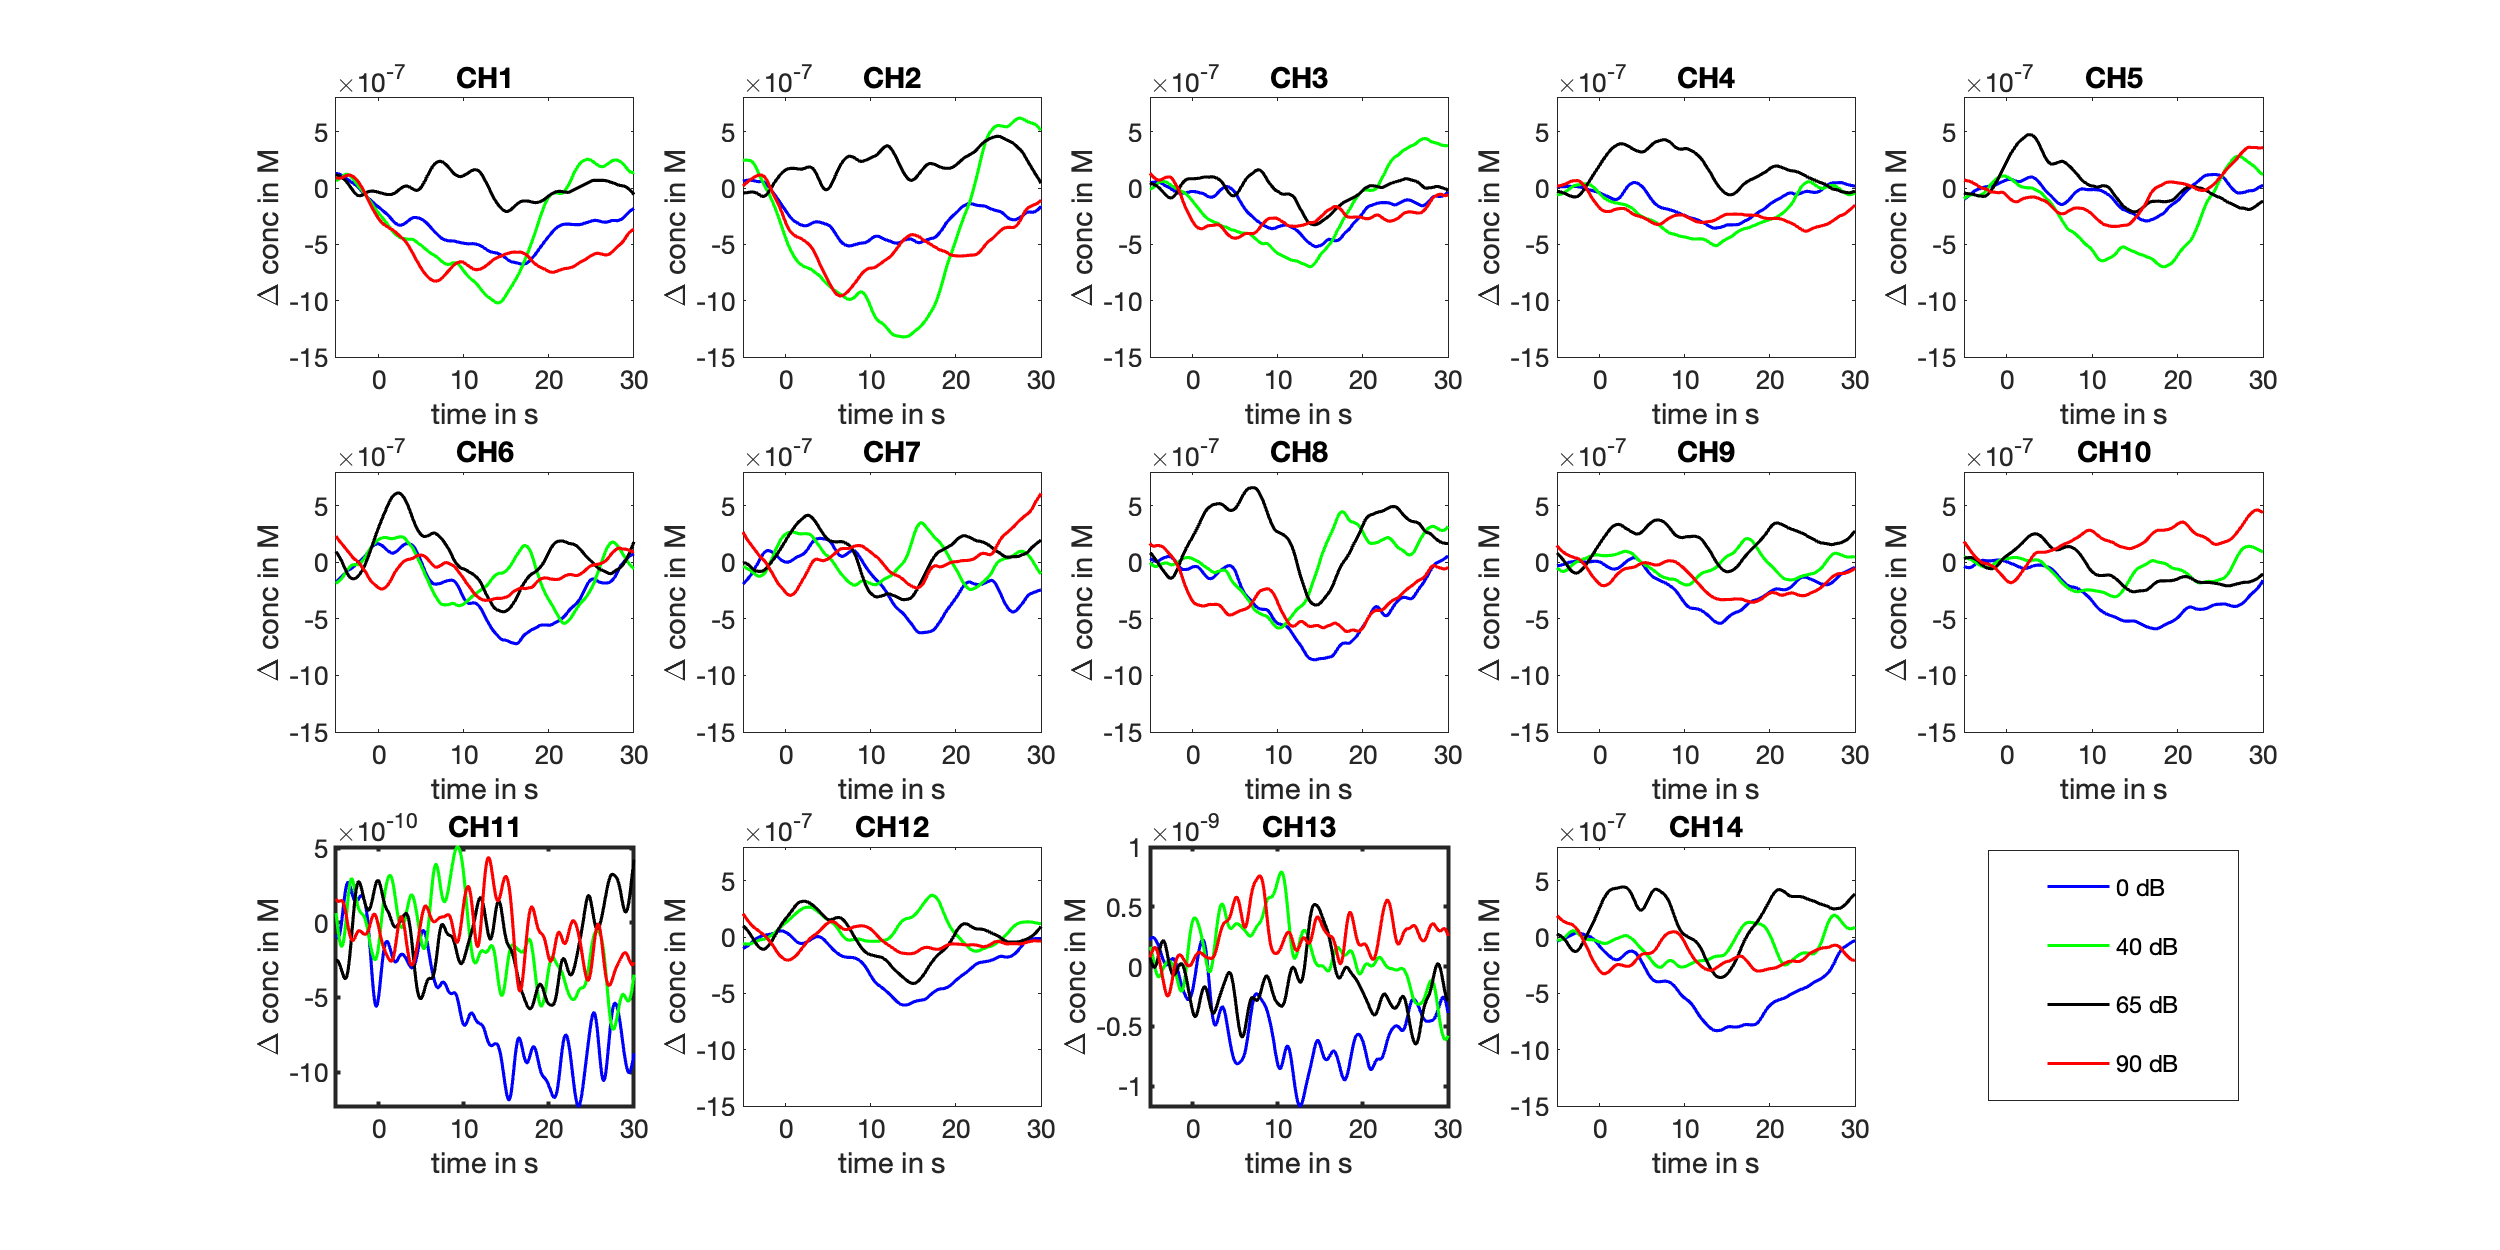
\includegraphics[scale=.4]{bilder/HbO_Mole/sub_luca2_s_HbO.png}
  \caption{HbO measurement from participant 8. Silent comparison}
  \label{fig:somesignal}
\end{figure}

\begin{figure}[H]
  \centering
    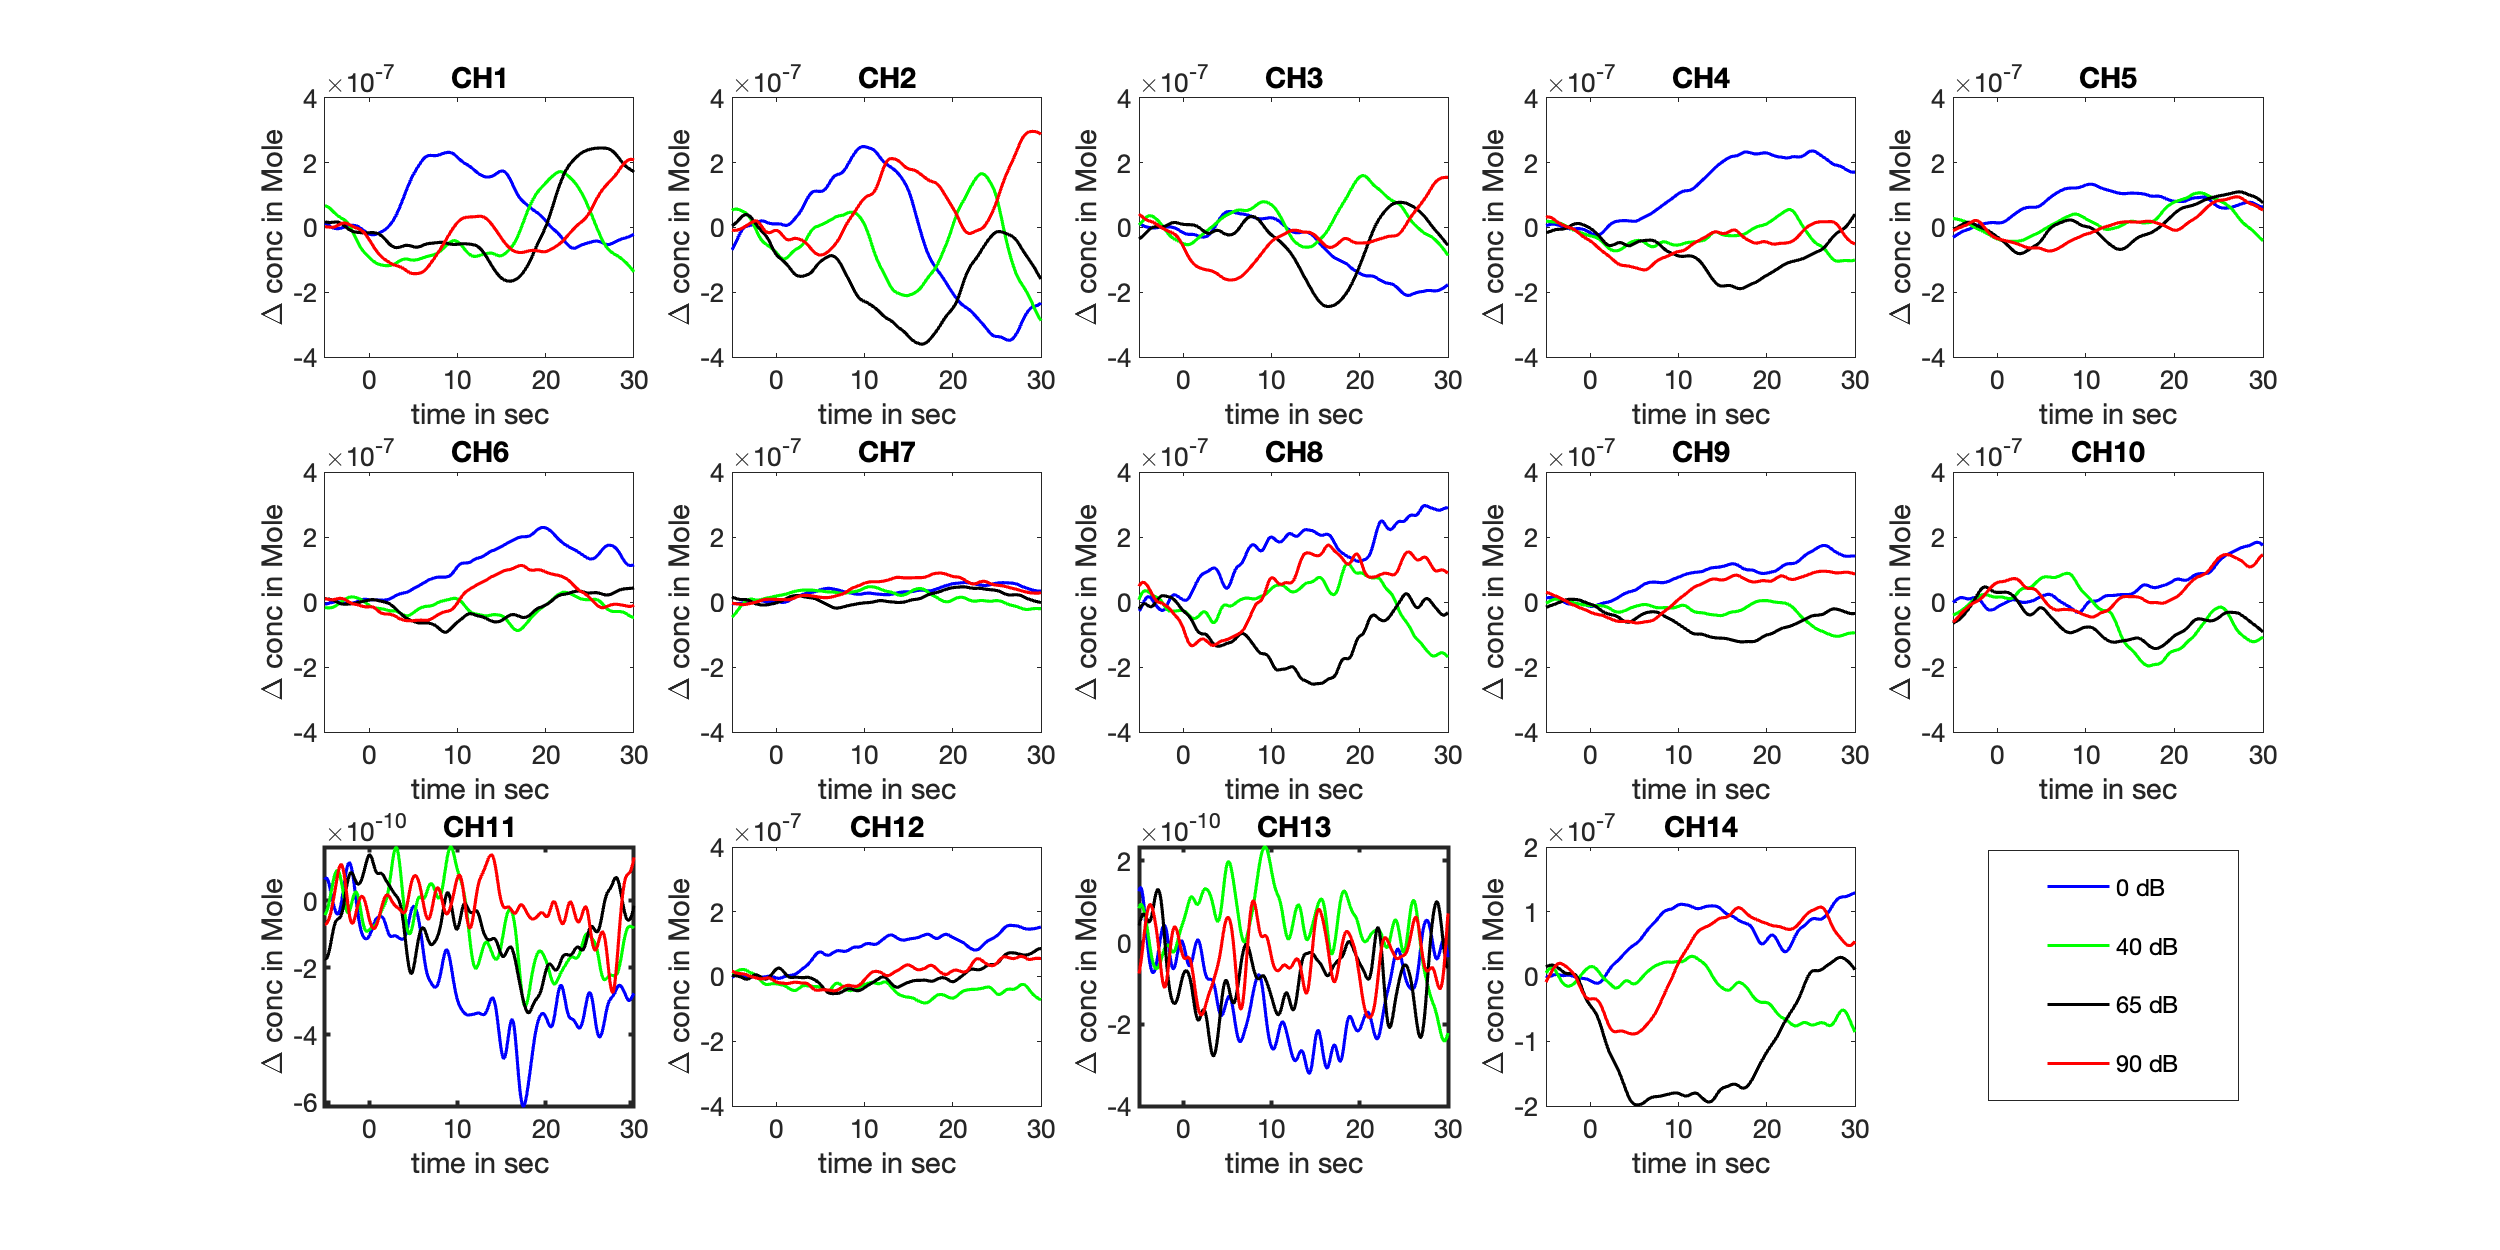
\includegraphics[scale=.4]{bilder/HbR_Mole/sub_luca2_s_HbR.png}
  \caption{HbR measurement from participant 8. Silent comparison}
\end{figure}

\begin{figure}[H]
  \centering
    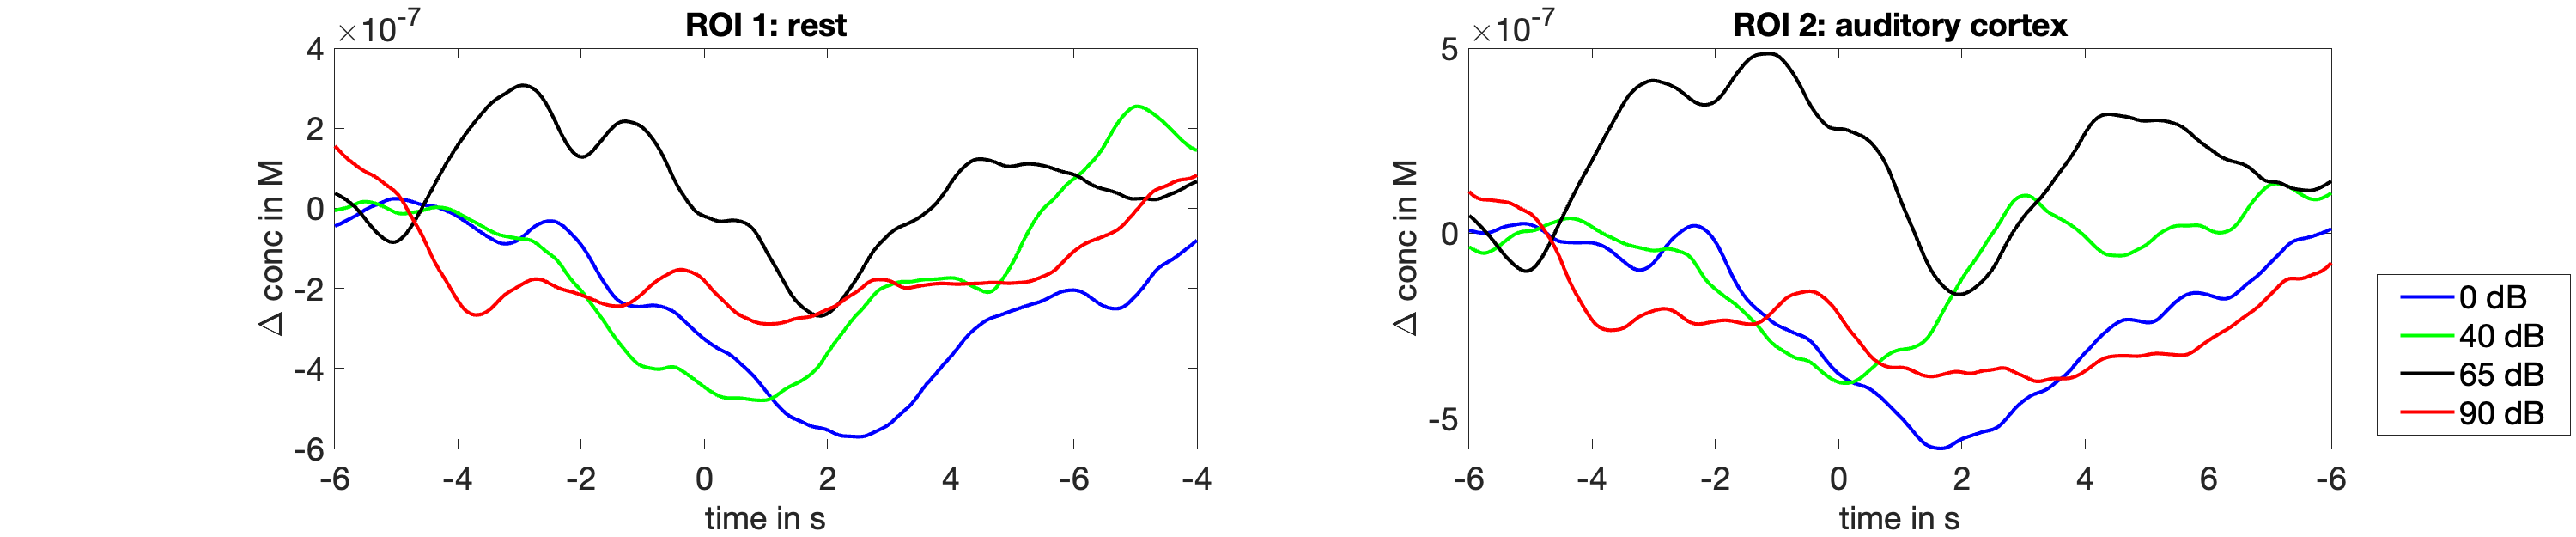
\includegraphics[scale=.29]{bilder/ROI/sub_luca2_s_HbO.png}
  \caption{ROI measurement from participant 8. Silent comparision.}
\end{figure}

This participant was given only silence stimuli. No pattern could be concluded for the measured waveform morphology. Nonetheless, it is noteworthy to know that even if there were almost no visual and sound stimuli, dynamic hemoglobin response still presented.